\documentclass[11pt, oneside]{article} 
\usepackage{geometry}
\geometry{letterpaper} 
\usepackage{graphicx}
	
\usepackage{amssymb}
\usepackage{amsmath}
\usepackage{parskip}
\usepackage{color}
\usepackage{hyperref}

\graphicspath{{/Users/telliott/Github/calculus_book/png/}}
% \begin{center} 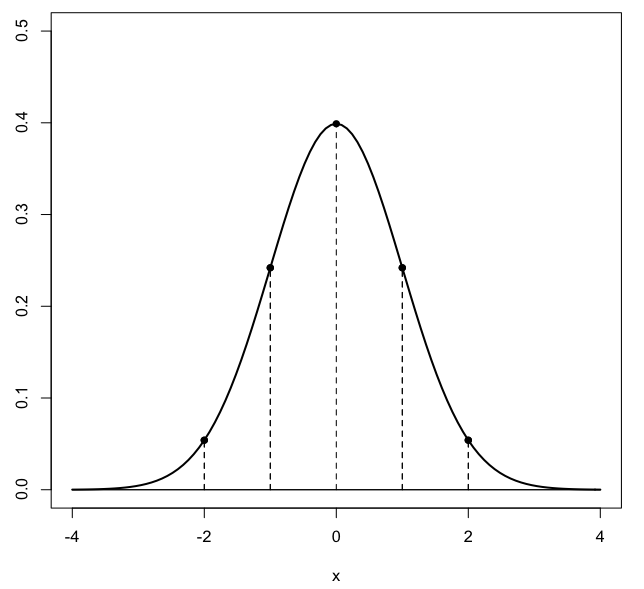
\includegraphics [scale=0.4] {gauss3.png} \end{center}

\title{Archimedes}
\date{}

\begin{document}
\maketitle
\Large

\subsection*{biography}

Archimedes is often ranked as the greatest of the Greek mathematicians.  He stands with Newton, Euler and Gauss, the best of the moderns.

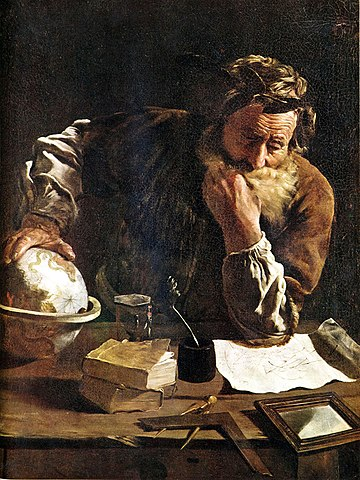
\includegraphics [scale=0.4] {archimedes_1620.jpg}
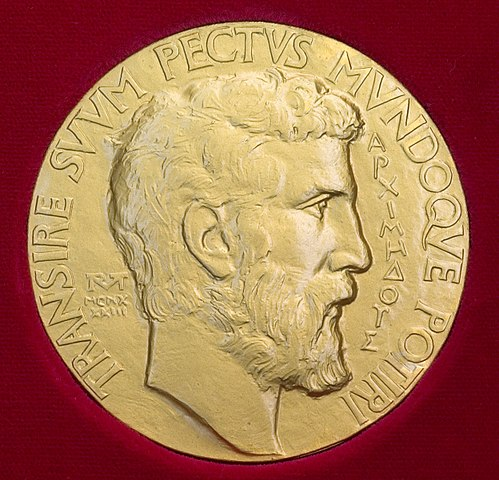
\includegraphics [scale=0.4] {archimedes_fields.jpg}

Here are two images, the first is a painting by Fetti from 1620 that is in the wikipedia article on Archimedes:

\url{https://en.wikipedia.org/wiki/Archimedes}

The other is the image on the famous Fields medal, which is sometimes described as the "Nobel prize" for mathematics.

\url{https://en.wikipedia.org/wiki/Fields_Medal}

Archimedes lived and died (c.287-212 BC) in the beautiful city of Syracuse, found on the southeastern coast of modern Sicily.  He is famous for many inventions, derivations and discoveries, but was evidently proud of the formula for the volume of the sphere. 

The very simple result is that the volume is two-thirds that of a cylinder that just encloses the sphere.  

Because he was so famous (perhaps so proud) of his discovery, there was a sculpture of the sphere and cylinder carved on his gravestone, near the Agrigentine gate of Syracuse.  The grave was found by the Roman orator Cicero, covered by brush after 137 years of neglect.  It is now lost again.

\subsection*{slices of solids}

The following is Archimedes simple but subtle argument.  

We compare a half-sphere and an inverted cone to a cylinder.  
\begin{center} 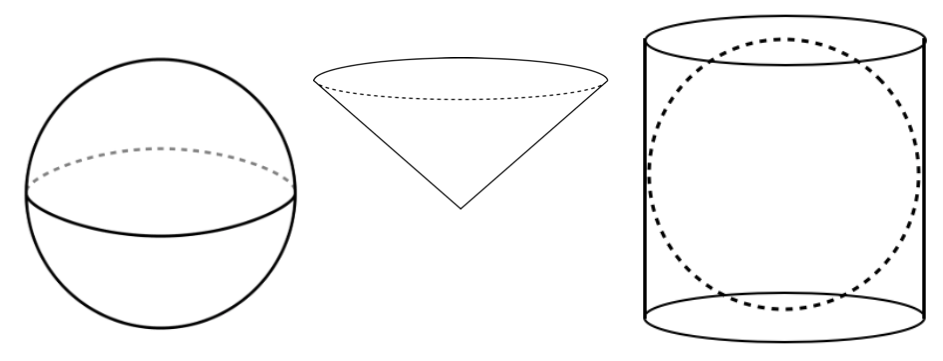
\includegraphics [scale=0.4] {scc1.png} \end{center}

Below is a diagram showing a \textbf{vertical} cross-section through the center of each solid so we can visualize the geometry.  The radius $R$ is the same for all three.  In addition, the cone and cylinder have overall height equal to $R$.

\begin{center} 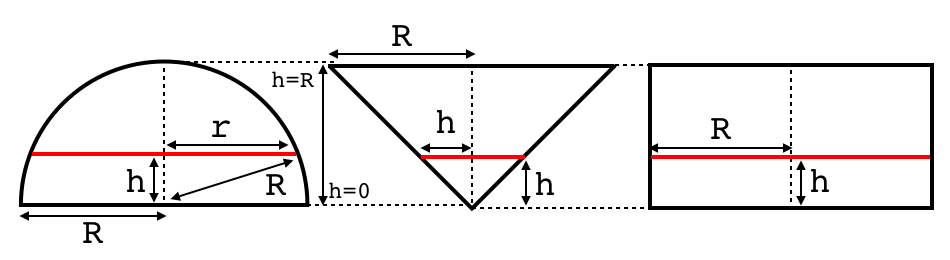
\includegraphics [scale=0.45] {scc2.png} \end{center}

Now, imagine making a \textbf{horizontal} slice through each solid at an arbitrary but constant height $h$, shown by the red lines.  I hope you can visualize each of these red slices, which are perpendicular to the page.  

Each slice is a circle.  Any cross-section of a sphere is a circle.  

For the cylinder and cone, cross-sections perpendicular to the central axis are circles as well.  

The question we ask is:  what is the area for each slice?

To answer that, we need to determine the radius for each red circle.  

Moving right-to-left, the radius of the cylinder is just $R$.  For the cone, the radius at each height $h$ is equal to $h$, since $R = H$.  And for the sphere, we use the Pythagorean theorem to find that
\[ r^2 + h^2 = R^2 \]
\[ r^2 = R^2 - h^2 \]

For more on this theorem see \hyperref[sec:pythagorean_thm]{\textbf{here}}.

The first insight of the proof is to recognize that the radius squared for the sphere's slice ($r^2$), plus the radius squared for the cone ($h^2$) is equal to $R^2$, the radius squared for the cylinder.

Since the area of each circle is proportional to to the radius squared (namely $A = \pi r^2$ and so on) and
\[ \pi r^2 + \pi h^2 = \pi R^2 \]
so the areas add too.  Our just famously and remarkable simple result:  \emph{sphere plus cone equals cylinder}.

\subsection*{invariance}

The second crucial insight of the proof is to recognize that this property is invariant, it does not depend on which height we choose to make the slice.  The three slices obtained at any height $h$ add up like this.  So if we imagine making a bunch of slices for each solid and adding them all up to find the volume, the volumes will add too.

This idea is now called Cavalieri's principle, though it was called the "method of indivisibles" before that.

The volume of the cylinder is simply $\pi R^3$.  The volume of the cone is known to be one-third the area of the base times the height, or $1/3 \ \pi R^3$.

Subtract to find that the area of the half-sphere is $2/3 \ \pi R^3$, and therefore the volume of the whole sphere is
\[ V_{\text{sphere}} = \frac{4}{3} \pi R^3 \]

There is a bit of a trick here to hide the idea introduced in calculus, which makes this thinking rigorous.  The sphere and cone have variable widths, which means that the radius will be different on the top of a slice compared to the bottom.  Therefore, the slices have to be made very thin.  In calculus they become infinitely thin, but we add up infinitely many of them.

Moreover, Archimedes was subject to certain limitations (discussed by Bressoud), which lead him to formulate the argument in terms of moments (masses of the solids and their centers).  I have left that complication out of this discussion.

\subsection*{knowledge before proof}

Archimedes said that he discovered the correct result by balancing the three objects on a fulcrum.  

According to Archimedes (in the Method, translation by Heath)

\begin{quote}For certain things which first became clear to me by a mechanical method had afterward to be demonstrated by geometry...\textcolor{blue}{it is of course easier, when we have previously acquired by the method some knowledge of questions, to supply the proof than it is to find the proof without any previous knowledge.} This is a reason why, in the case of the theorems the proof of which Eudoxus was the first to discover, namely, that the cone is a third part of the cylinder, and the pyramid a third part of the prism, having the same base and equal height, we should give no small share of the credit to Democritus, who was the first to assert this truth...though he did not prove it.
\end{quote}

From his description, what Archimedes actually balanced is a set-up like that shown below:

\begin{center}
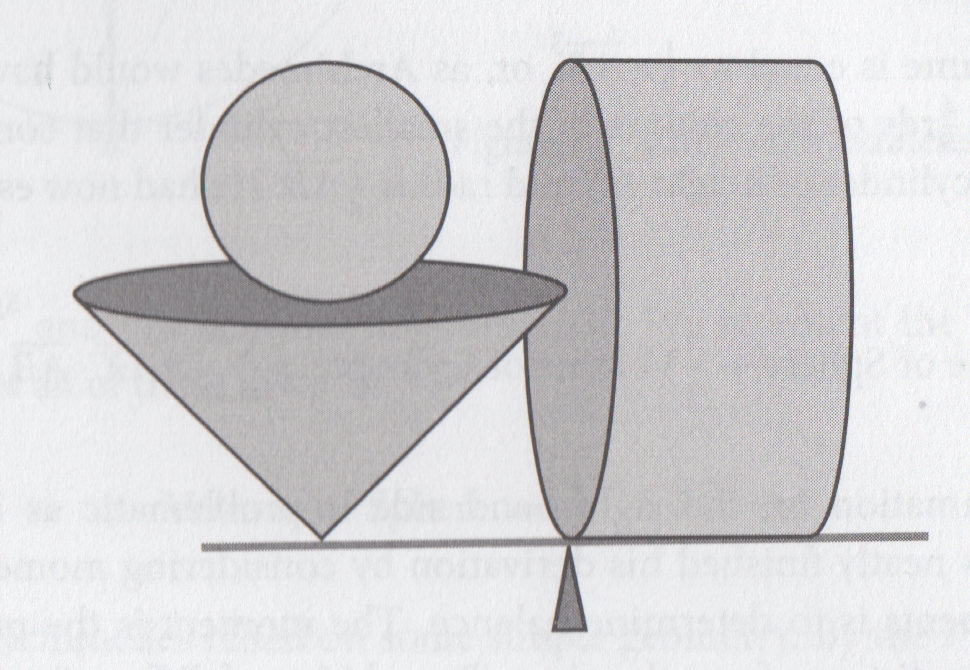
\includegraphics [scale=2.0] {archimedes2.png}
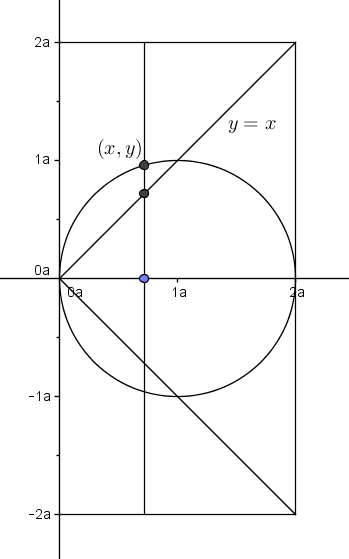
\includegraphics [scale=0.5] {SphereVolume.png}
\end{center}

\url{https://proofwiki.org/wiki/File:SphereVolume.png}

We have a:

$\circ$ \ sphere with radius $R$

$\circ$ \ cone with radius $2R$ and height $2R$

Their combined volumes:
\[ V = \frac{4}{3} \ \pi R^3 + \frac{1}{3} \ \pi (2R)^2 \cdot 2R \]
\[ = \frac{12}{3} \ \pi R^3 = 4\pi R^3\]

balanced against

$\circ$ \ a cylinder with radius $2R$ and height $2R$ with 
\[ V = \pi (2R)^2 \cdot 2R = 8 \pi R^3 \]

However, the moment of the cylinder is at one-half the distance from the fulcrum as that of the sphere-cone combination, so it balances.

\end{document}